\documentclass[12pt]{ctexart}

\usepackage{stfloats}
\usepackage{enumitem}
\usepackage[linesnumbered,ruled,vlined]{algorithm2e}
\usepackage{geometry}
\usepackage{booktabs}
\usepackage{graphicx}
\usepackage[final]{pdfpages}
\usepackage[stable]{footmisc}
\usepackage{threeparttable}
\usepackage{indentfirst}
\usepackage{minted}
\usepackage{listings}
\usepackage{xcolor}
\usepackage{subfigure}
\usepackage{amsmath}
\DeclareMathOperator*{\argmin}{arg\,min}
\usepackage{amsfonts}
\usepackage{hyperref}
\usepackage{cleveref}
\crefformat{figure}{#2图~#1#3}
\crefrangeformat{figure}{图~(#3#1#4)\;\~{}\;(#5#2#6)}
\crefmultiformat{figure}{图~(#2#1#3)}{和~(#2#1#3)}{,(#2#1#3)}{和~(#2#1#3)}

% \setlength{\parindent}{0pt}
\geometry{top=25mm,bottom=25mm,left=25mm,right=25mm}
\lstset{
    basicstyle=\tt,
    basicstyle=\small,
    keywordstyle=\color{purple}\bfseries,
    rulesepcolor= \color{gray},
    breaklines=true,
    numbers=left,
    numberstyle= \small,
    commentstyle=\color{gray},
    frame=shadowbox
}

\hypersetup{
    colorlinks=true,
    linkcolor=blue,
    filecolor=magenta,
    urlcolor=cyan,
}
\urlstyle{same}

\title{组合优化论文(阅读体会)}
\author{杜睿}
\date{}

\begin{document}
\tableofcontents
\maketitle

\section{概述}
组合优化问题,或者说优化问题,有两条主线,一是问题的建模,解的编码与表示,
二是最优化算法,平衡局部最优的开采(邻域搜索)和全局最优的探索(跳坑策略)。
如果开采不足,收敛性不好,解的质量堪忧;如果探索不够,容易早熟,陷入局部最优解。

许多优化问题无法在多项式时间内求的最优可行解,
对于这样的问题,研究的重点落在近似算法,
即设计一套算法,能在较短时间内,
给出相当接近最优解的一个近似可行解。

可以按照是否引入随机性,可以将近似算法,分为非随机近似算法和随机型近似算法。
也可以按照算法的通用性,将部分启发算法划归为万用元启发算法,例如模拟退火等。

对于近似算法而言,有两类评价指标:
第一种是理论分析,在理论上证明,
最坏情况下近似比(算法所得目标函数值与最优目标函数值之比)不超过某个常数;
第二种是实例分析,对于某些启发算法而言,不具有最坏情况下,理论的近似比保证,
于是选择特定的测试用例,
在相同环境、硬件配置下,对比该算法与其他算法的优劣(求解速度与求解质量)。

对于组合优化而言,与实值优化相比,目标函数及其决策变量在高维表示中,往往是离散、不可导的;
如果要借鉴实值优化方法,如“梯度下降”,则要定义解的“邻域”。

对于非凸的优化问题,既要能找到“最优”,也要能跳出较差的“局部最优”。

\section{求解旅行商问题的近似算法}

\subsection{问题描述}

给定一个有向完全图$G=(V,A)$,
其中集合$V=\{v_1,\dots,v_n\}$是顶点集合,
每个顶点代表一个城市,
$n$是顶点数($n \ge 3$),
集合$E=\{(v_i,v_j) | v_i,v_j \in V,v_i \ne v_j\}$是有向边集合。
$c_{ij}$是有向边$(v_i,v_j)$的长度(权值),
$c_{ij}$是已知的正实数且满足$c_{ij}=c_{ji}$,
其中$(v_i,v_j)\in E$。
集合$\Sigma$是顶点全排列的集合,
共有$n$!元素。
$\sigma$是所有顶点的一个全排列:$\sigma=(\sigma(1),\dots,\sigma(n))$,$\sigma \in \Sigma$,
$\sigma(i)\in V (1\le i \le n)$。
$\sigma$对应着一条历经所有顶点的回路:
从顶点$\sigma(1)$走到顶点$\sigma(2)$,$\cdots$,
从顶点$\sigma(n-1)$走到顶点$\sigma(n)$,
从顶点$\sigma(n)$回到顶点$\sigma(1)$。

全排列$\sigma$所对应的回路的长度记为$L(\sigma)$,
$L(\sigma) = \sum\limits_{{i=2}}^{n} c_{\sigma(i-1) \sigma(i)} + c_{\sigma(n) \sigma(1)}$。

目标是给出所有顶点的一个全排列$\sigma^\star$,
使得$L(\sigma^\star)= \mathop{\min}\limits_{{\sigma \in \Sigma}} L(\sigma)$。

\subsection{算法描述}

旅行商问题的经典近似算法是克里斯托菲德斯算法,它在理论上保证最差情况下近似比不超过1.5。
王磊老师在课上跟学生们讲过一个随机型近似算法(下文称王磊算法)。

基本算法$B_0$描述如下:

\begin{description}
    \item[输入:] 指导序列$\gamma$,$\gamma$是所有顶点的一个全排列;
    \item[开局:] 用$\gamma$前$3$个点绘制外接凸多边形(三角形),构成初始回路$\sigma = (\gamma(1), \gamma(2), \gamma(3))$;
    \item[迭代:] 每次从当前格局向新格局演化时,取出下一个点,按照使得新的部分回路长度尽量短的贪心策略,将其插入至$\sigma$合适的位置;
    \item[停机:] 直至产生$n$个点的回路$\sigma$,算法结束,输出$\sigma$。
\end{description}

算法伪代码如下,输入一个指导序列,输出一条回路。

\IncMargin{1em}
\begin{algorithm}[H]
    \SetKwInOut{Input}{input}\SetKwInOut{Output}{output}
    \Input{$V=\{v_1, \ldots, v_n\}, dist(\cdot, \cdot), \gamma$ a permutation of $V$}
    \Output{$\sigma$ the tour}
    \BlankLine
    $\sigma \leftarrow (\gamma(1), \gamma(2), \gamma(3))$\;
    \For{$i \leftarrow 4$ \KwTo $n$}{
        $best\_idx \leftarrow \argmin\limits_{j \in \{1, \ldots, |\sigma|\}}  L(\sigma_{1:j}) + dist(\gamma(i), \sigma(j)) + L(\sigma_{j:|\sigma|}) - L(\sigma) $\;
        $\sigma \leftarrow (\sigma_{1:best\_idx}, \gamma(i), \sigma_{best\_idx+1:|\sigma|})$\;
    }
    \caption{WangLei $B_0$ Algorithm}
\end{algorithm}
\DecMargin{1em}

从在线算法的视角来看,指导序列其实表达的是城市到达先后顺序,
城市到达的先后顺序不同,即使是相同的在线算法,所求的回路的长度也是不同的。

考虑对所有指导序列$\gamma \in \Gamma$,目标是$\gamma^\star = \argmin\limits_{\gamma \in \Gamma} L(A_1(\gamma))$。

据此,王磊老师在基础回路算法$B_0$的基础上,提出算法$A_0$:

\begin{description}
    \item[初始格局:]初始化$\gamma$,通过$A_1$算法指导获得回路$\sigma = A_1(\gamma)$,以及长度$l = L(\sigma)$;
    \item[邻域搜索:]邻域变换得到$\gamma^\prime$、$\sigma^\prime$及$l^\prime$,若$l^\prime < l$,依照最陡下降法,更新格局$\gamma \leftarrow \gamma^\prime$
    \item[跳坑策略:]当$\gamma$位于局部最优,即几乎尝试所有邻域都无法改善目标函数时,重新随机初始化$\gamma$或者采用大步长算子(如块移动、块对换、块插入)对$\gamma$进行变换。
\end{description}

\begin{algorithm}[H]
    \SetKwInOut{Input}{input}\SetKwInOut{Output}{output}
    \Input{$V, dist(\cdot, \cdot), L(\cdot), epoch, early\_stop$ \\
        $permutation(\cdot), transform(\cdot), shuffle(\cdot)$}
    \Output{$\sigma, l$}
    \BlankLine
    $\gamma \leftarrow permutation(V)$; $\sigma \leftarrow A_1(\gamma)$; $l \leftarrow L(\sigma)$\;
    \For{$e \leftarrow 1$ \KwTo $\text{epoch}$}{
        $\gamma^\prime \leftarrow transform(\gamma)$; $\sigma^\prime \leftarrow A_1(\gamma^\prime)$; $l^\prime \leftarrow L(\sigma^\prime)$\;
        \If{$l^\prime < l$}{
            $\gamma \leftarrow \gamma^\prime$; $\sigma \leftarrow \sigma^\prime$; $l \leftarrow l^\prime$\;
        }
        \If{no improvement for \text{early\_stop} iterations}{
            $\gamma \leftarrow permutation(V)$ or $\gamma \leftarrow shuffle(\gamma)$\;
        }
    }
    % $\sigma^* \leftarrow \sigma$; $l^* \leftarrow l$\;
    \caption{WangLei $A_1$ Algorithm}
\end{algorithm}

$A_1$是一个随机型近似算法,对于初始化不同的$\gamma$,算法的输出有可能是不同的。

对于$B_0$算法的开局,可以将$3$个点,替换为$m$个点。即:

\IncMargin{1em}
\begin{algorithm}[H]
    \SetKwInOut{Input}{input}\SetKwInOut{Output}{output}
    \Input{$V=\{v_1, \ldots, v_n\}, dist(\cdot, \cdot), \gamma$ a permutation of $V$, $m$}
    \Output{$\sigma$ the tour}
    \BlankLine
    $\sigma \leftarrow$ a convex hull of points $\gamma$ using Graham's Scan Algorithm\;
    \For{$i \leftarrow m+1$ \KwTo $n$}{
        $best\_idx \leftarrow \argmin\limits_{j \in \{1, \ldots, |\sigma|\}}  L(\sigma_{1:j}) + dist(\gamma(i), \sigma(j)) + L(\sigma_{j:|\sigma|}) - L(\sigma) $\;
        $\sigma \leftarrow (\sigma_{1:best\_idx}, \gamma(i), \sigma_{best\_idx+1:|\sigma|})$\;
    }
    \caption{WangLei $B_1$ Algorithm}
\end{algorithm}
\DecMargin{1em}

\subsection{感悟体会}
王磊算法的创新、启发意义主要是能将组合优化的两条主线结合起来:

\begin{enumerate}
    \item 传统启发算法求解旅行商问题,几乎全部都是直接在回路$\sigma$上进行邻域扰动,获得新解。而王磊算法则提出了$\gamma \to \sigma$的映射算法$A_1$,这相当于对原有解空间进行了“扭曲”,将求“回路”的原问题转化为了求“指导顺序“的新问题。

          最优化理论中,原始问题很难求解时,往往通过引入对偶问题的方式,简化对原始问题的求解。在机器学习中,也有代替函数、核函数作为例子。但是,我们不禁要问,对于所有的“指导序列”$\gamma \in \Gamma$,它们所生成的所有回路集合$\Sigma^\star$,是否包含了最优回路$\sigma^\star$?

          即,通过指导序列将问题转换,问题转换前后是否仍然具有“一致性”  ?

    \item 邻域搜索和跳坑策略思想并不高深。局部极小值的定义来自于函数求极值,跳坑则更有烟火气:如果你已经期末总评满分了,就要跳坑,到更有希望的学府继续深造。

          无论是回路$\sigma$还是指导序列$\gamma$都是高维空间的一个点,若其邻域中的“点”所对应的回路长度都不比中心点短,则该中心点是局部极小值点;当邻域搜索陷入局部极小值点时,就应该采用“跳坑策略”,进行随机扰动,跳出陷阱,继续邻域搜索。

          这其中的问题有二:一是“随机扰动”算子和所谓“邻域算子”在本质上究竟有何不同?设计的“邻域算子”真的在逻辑上只是轻微的扰动吗?二是随着邻域算子设计的不同,邻域中的“点”随着维度的增大,个数可能比想象中要多得多,因此有时候又不得不采用固定次数的方式来执行邻域搜索,导致邻域开采不足。邻域搜索对应“变异”、“开采”,而跳坑策略则对应“探索”,可以说所有的最优化算法都要考虑这两者的平衡。

    \item 生成回路算法本身也具有烟火气。想象一下,借一个扎头发的橡皮筋,套住几个点;然后采用贪心策略,将其余点加入回路。

          传统的最近邻点贪心策略是,最后一步方能连成回路,这就导致目光浅显、虎猴蛇尾;而如果是在一个成形的“回路”中添加,每次添加评价的都直接是回路的全长,则能一定程度上缓解“短视”问题。
          这启发我们同样是贪心策略,但是如何运用,运用的好不好是可以评价的,是有优劣的;此外,要习惯从生活中获得启发,不要学死了。
\end{enumerate}

\section{求解SAT问题的拟物方法}

\subsection{问题描述}

给一命题逻辑公式,问是否存在一组变元赋值使该公式为真,即该命题是否可满足。
因为任何命题逻辑公都可以写作合取范式(\textbf{C}lausal \textbf{N}ormal \textbf{F}orm)的形式;
因此,我们只研究合取范式的可满足性问题。如下是一个具体问题实例,有5个逻辑变元(Literal,文字):

$$(A \vee B \vee C) \wedge (B \vee \neg C \vee \neg F) \wedge (\neg B \vee E)$$

$(A \vee B \vee C)$、$(B \vee \neg C \vee \neg F)$、 $(\neg B \vee E)$是子句(Clause);
我们将使得命题逻辑公式为真的一组逻辑赋值称为一个世界模型(World Model)。
为了证明这一逻辑命题公式的可满足性或不可满足性,可采取真值表方法枚举所有可能情况,共有32行:

\begin{table}[htbp]
    \caption[1]{真值表法}
    \centering

    \begin{threeparttable}
        \begin{tabular}{cccccc}
            \toprule
            $I(A)$   & $I(B)$   & $I(C)$   & $I(E)$   & $I(F)$   & Statement \\
            \midrule
            False    & False    & False    & False    & False    & False     \\
            False    & False    & False    & False    & True     & False     \\
            False    & False    & False    & True     & False    & False     \\
            False    & False    & False    & True     & True     & False     \\
            $\cdots$ & $\cdots$ & $\cdots$ & $\cdots$ & $\cdots$ & $\cdots$  \\
            True     & True     & True     & False    & False    & False     \\
            True     & True     & True     & False    & True     & False     \\
            True     & True     & True     & True     & False    & True      \\
            True     & True     & True     & True     & True     & True      \\
            \bottomrule
        \end{tabular}
    \end{threeparttable}
    \qquad
\end{table}

\subsection{经典算法}

\subsubsection{Davis-Putnam算法}

任一变元取值为零或一(两种情况),
每个文字之间的取值看似相互独立,
故对于$n$变元的SAT问题而言,
共有$2^n$种赋值方式。
真值表法是
首先枚举出来所有可能的赋值情形,
然后开始对于每一种赋值,核对在该赋值下,命题逻辑公式的真假值:
如果为真,则算法停机,该命题逻辑公式是可满足的;如果考虑所有可能的赋值,
均无法使得命题逻辑公式为真,则称该命题逻辑公式是不可满足的。
显然,这是一个确定性算法,时间复杂度为$O(2^n)$。

即使用深度优先搜索实现,
从制表逻辑的角度说,
因为表有$2^n$行,我们没有“跳行”,
我们没有设计任何机制,减小问题规模或搜索空间。

于是,有人思考在实现深度优先搜索时,
如何“减枝”,如何“减小问题规模”。

\begin{figure}[htbp]
    \centering
    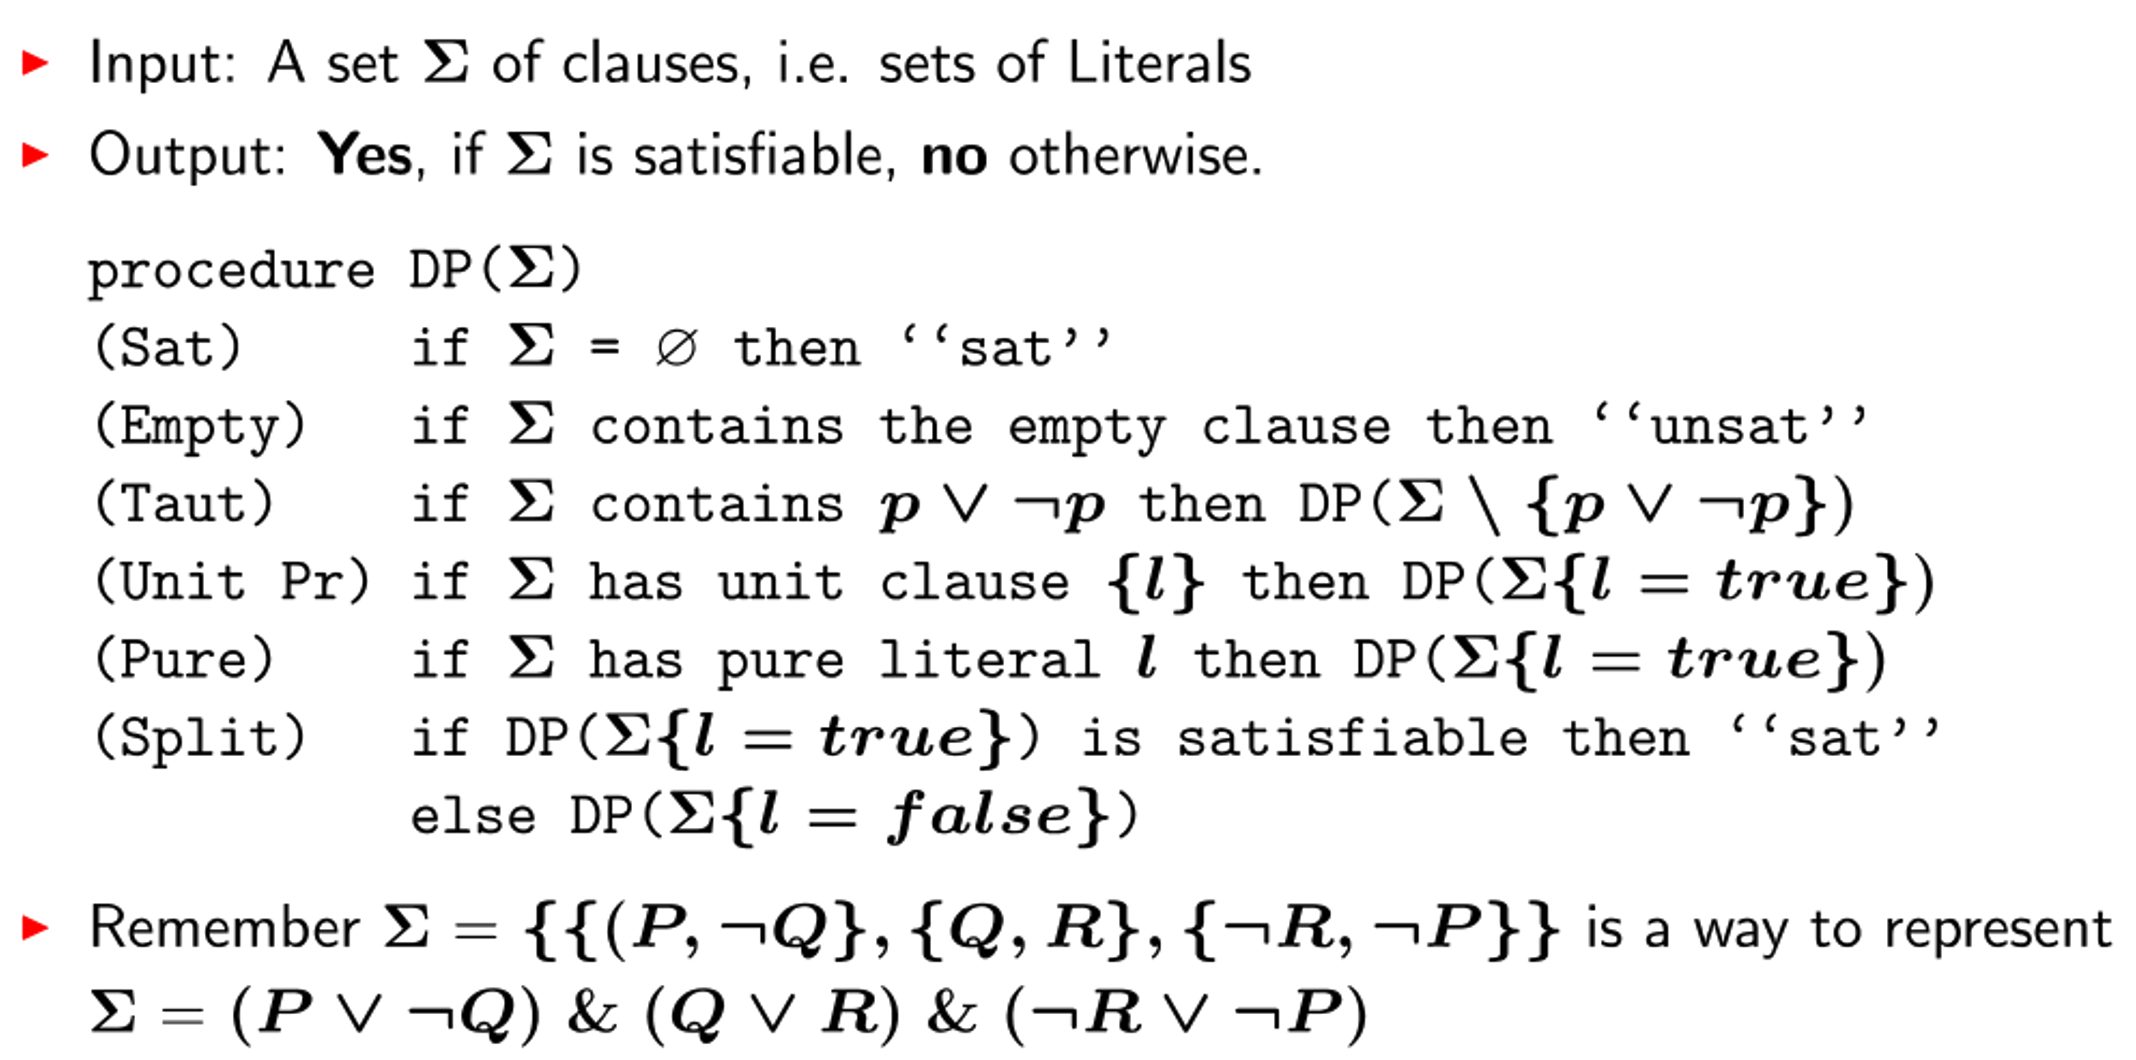
\includegraphics[width=0.9\linewidth]{dp.png}
    \caption{Davis-Putnam算法伪代码}
\end{figure}

首先,考虑基本情况和终止条件:
\begin{enumerate}
    \item 如果所有子句均被消去,则当前输入的命题逻辑公式可满足;
    \item 如果一个子句未被消去,但其中所有变元均被消去,则说明该子句无法满足;
    \item 如果一个子句中包含重言式,则可以消去,减小问题规模递归;
    \item 如果一个逻辑命题中,存在一个逻辑变元,仅在一个子句中出现,我们可以将其赋值为真,消去所在子句,减小问题规模递归;
\end{enumerate}

然后,考虑下探回溯:这是一个传统子集型深度优先搜索问题,
选择一个逻辑变元赋值为真,简化逻辑命题公式之后,在子问题上递归;
如果无法满足,再回溯,选择该逻辑变元为假,然后在子问题上递归,最后一定会进入终止条件。

最坏情况下,该算法的时间复杂度依然为$O(2^n)$。
但是,我们早已在OJ上见过,用优先队列式分支限界法解决0-1背包问题,并不比所谓的动态规划要差多少。

这意味着,我们在评价算法好坏时,
要从理论上分析最坏情况,
但同时又要认识到现实生产实际上,如芯片制造业,
可能最坏情况发生的概率极小。
因此,我们在评价Davis-Putnam算法时,
并不能说它是毫无贡献,白费功夫的。

\subsubsection{Clause-Learning法}

Davis-Putnam算法的提出显然是基于 算法设计与分析的经典设计哲学————分而治之,减小问题规模。

Clause-Learning是。 微软亚洲研究院Lintao Zhang的工作。 如果让我来解释,他用的自然是“拟人”策略。人看到一个问题,并非总是
要想着如何减小问题规模,但是也要时不时从错误中吸取教训、总结复盘, 即,从现有的失败案例中总结概括出更精炼的规则、道理,
这看似是增加当前的问题规模,但是,我们依然可以 通过增加子句的方式能够辅助剪枝。

\begin{figure}[htbp]
    \centering
    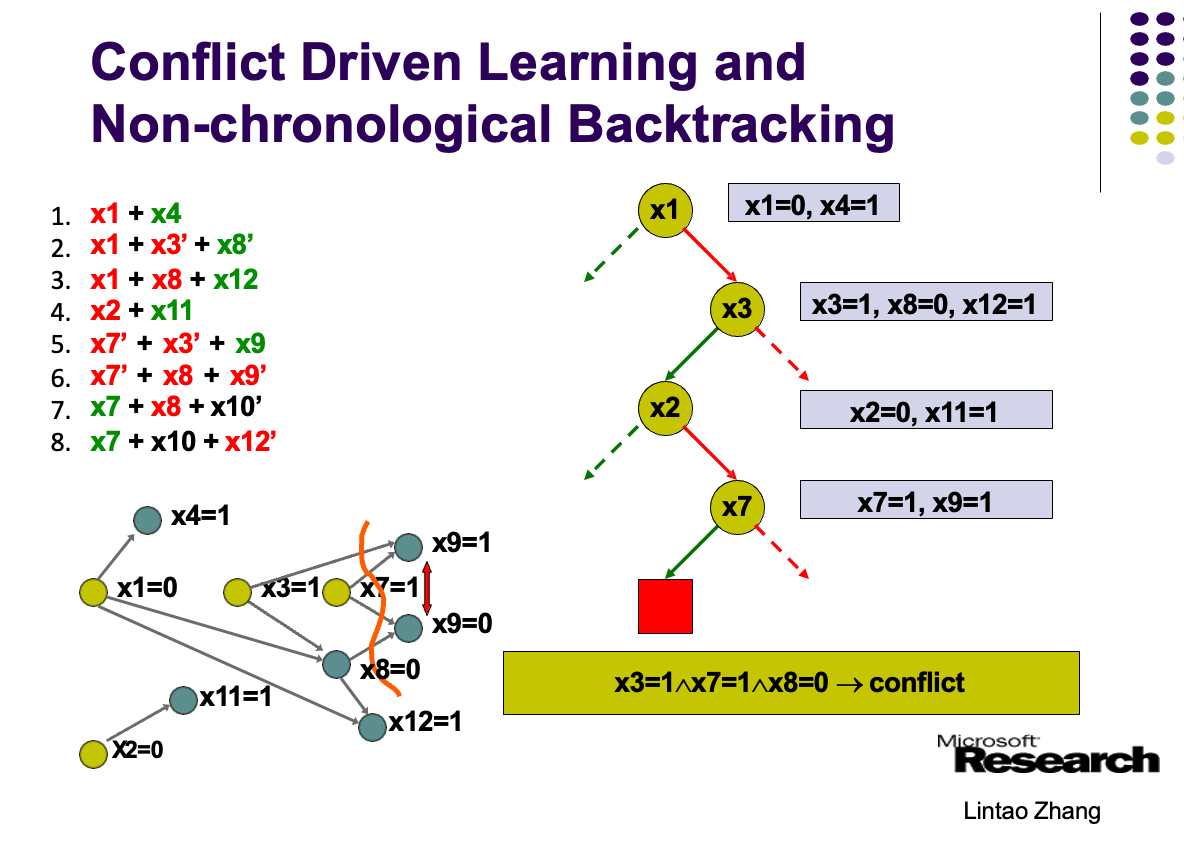
\includegraphics[width=\linewidth]{cl.png}
    \caption{规则学习算法举例}
\end{figure}

它记录一个赋值的依赖图,每次递归走入死胡同时,
将导致冲突的一组赋值作为一个子句,直接添加至原问题中
,这样的好处是,不会重复跳进同一死胡同。

注意,一般而言我们在理解算法设计哲学时,都会以为,只能减小问题规模,不能增大问题规模。
但是,不能学死了。这里看似增大了问题的规模,实则隐式的增加了递归出口
,达到剪枝的目的。

\subsection{Solar算法}

Solar算法的启发意义在于, 找到了一个问题的物理表式。

这个物理表示,首先是将非最优化问题,转换成了最优化问题。

我们都知道,世界是熵增的,
最后,物体都会处于势能最小的地方,
而这就是等效最优化问题的最小值。

SAT问题本身并不是一个”最优化“问题,
因为它要么是可满足,要么不可满足,
是非黑即白的, 没有”目标函数“。

有学者考虑MAXSAT问题,即将满足的子句个数作为目标函数。

但是,如果我们将原问题转换为物理表示,
目标函数则十分自然,那就是考虑电势能。

这种依柯西梯度法求总势能函数的最小值点的迭代过程,
事实上吻合于物理世界中那个带正电荷的质点走向最低势能位置的运动过程。

其次,这个物理表示将离散的组合优化问题,转换为了连续的实值优化问题。

玻璃珠一旦进入某钢板后此钢板由于屏蔽现象的原因即失去引力,待到又离开这块钢板了,则此板又对珠子恢复引力,再次将其引向自身;即考虑玻璃珠的坐标。


\end{document}

% \begin{figure}[htbp]
%     \centering
%     \includegraphics[height=550pt]{v1-class-compat.png}
%     \caption{UML类图(第二版)}
% \end{figure}

% \begin{minted}[mathescape,
%     linenos,
%     numbersep=5pt,
%     frame=lines,
%     gobble=4,
%     framesep=2mm]{Java}
%     public interface Observable {
%         void attachObserver(Observer o);

%         void detachObserver(Observer o);

%         void notifyObservers();
%     }
% \end{minted}

% \begin{lstlisting}[language={java},caption={收容队列(基于响应比的优先队列)}]
% private PriorityQueue<Task> queue = new PriorityQueue<>(new Comparator<Task>() {
%     @Override
%     public int compare(Task o1, Task o2) {
%         return (o2.getResponseRate(Clock.minutes) - o1.getResponseRate(Clock.minutes) > 0) ? (1) : (-1);
%     }
% });
% \end{lstlisting}